\documentclass[border=10pt]{standalone}
\usepackage{pgfplots}
\usepgfplotslibrary{colormaps}
\pgfplotsset{compat=1.18}

\begin{document}
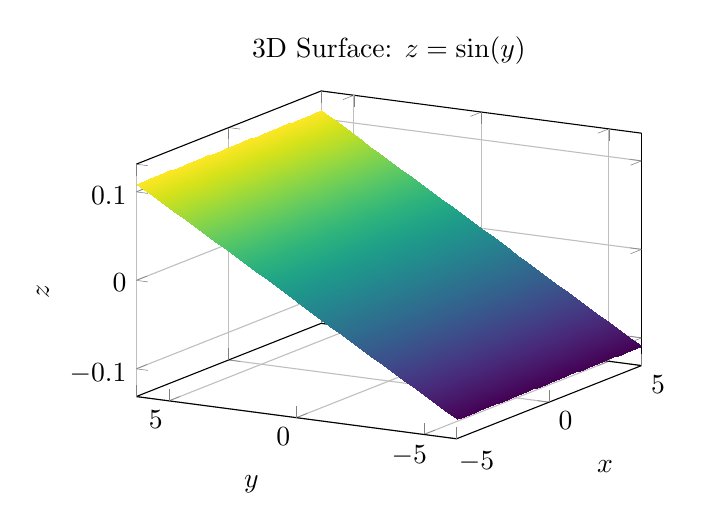
\begin{tikzpicture}
\begin{axis}[
    xlabel={$x$},
    ylabel={$y$},
    zlabel={$z$},
    title={3D Surface: $z = \sin(y)$},
    view={-60}{20},
    colormap/viridis,
    grid=major,
    width=8cm,
    height=6cm,
]
\addplot3[
    surf,
    shader=interp,
    domain=-5:5,
    y domain=-2*pi:2*pi,
    samples=40,
    samples y=40,
] {sin(y)};
\end{axis}
\end{tikzpicture}
\end{document}